%
%  progress-presentation.tex
%  src
%
%  Created by Illya Starikov on 09/16/17.
%  Copyright 2017. Illya Starikov. All rights reserved.
%

% \documentclass[notes,xcolor=dvipsnames]{beamer}       % print frame + notes
% \documentclass[notes=only,xcolor=dvipsnames]{beamer}  % only notes
\documentclass[xclolor=dvipsnames]{beamer}            % only frames
%\documentclass[handout,xclolor=dvipsnames]{beamer}    % only frames, no pauses
\usepackage{soul,graphics}

\usepackage{amssymb,amsmath,verbatim,graphicx,microtype,upquote,units,booktabs,akkwidepage}

\newcommand{\chapterNumber}[1]{
    \setcounter{section}{#1}
    \addtocounter{section}{-1}
}
\title{Productivity (Presentation \#8)}
\subtitle{Special Topics (CS3001)}
\author{Illya Starikov}
\date{Sometimes In The Future}
\institute{Missouri University of Science and Technology}

\begin{document}
\begin{darkframes}
    \maketitle

    \begin{frame}
        \frametitle{A Brief Introduction}

        I knew this semester was going to be difficult. I decided I needed better time and assignment management. After some research, I decided I wanted to learn how to practice Getting Things Done (GTD).
    \end{frame}

    \begin{frame}
        \frametitle{A Brief Introduction}

        Getting Things Done is a time management method created by David Allen in 2001. It centers around the idea of planning actionable items in an external system. This allows the person following the program to not ponder on next actions, since they have all of them in front of them. The Getting Things Done lifestyle can best be described by David Allen in his own book, \href{https://www.amazon.com/Getting-Things-Done-Stress-Free-Productivity/dp/0142000280}{Getting Things Done: The Art of Stress Free Productivity}.
    \end{frame}

    \begin{frame}
        \frametitle{A Brief Introduction}

        As part of the Getting Things Done lifestyle, I need some sort of system to store all of my actions in. After \textit{a lot} of research and experimenting, I landed on \href{https://www.omnigroup.com/omnifocus}{OmniFocus}. It got by far the best reviews.
    \end{frame}

    \begin{frame}
        \frametitle{A Brief Introduction}

        \begin{figure}[H]
            \centering
            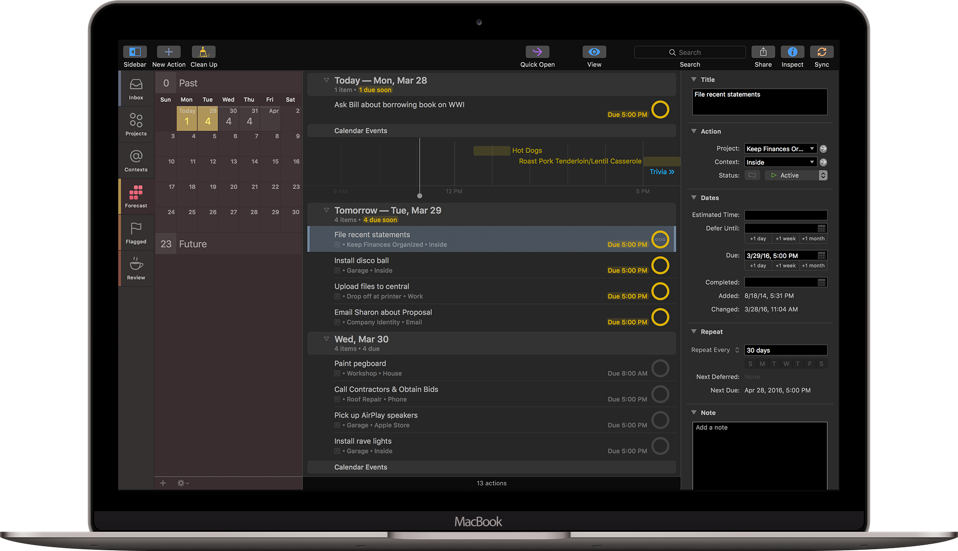
\includegraphics[width=.9\linewidth]{assets/omnifocus.png}
            \caption{OmniFocus On The Mac}
            \label{fig:OmniFocus}
        \end{figure}

    \end{frame}


    \begin{frame}
        \frametitle{Prior Knowledge}

        \begin{itemize}
            \item I was always interested in productivity, reading books such as The Power of Full Engagement and The Seven Habits of Highly Effective People.
            \item However, I never considered creating a system for all my actions.
        \end{itemize}
    \end{frame}

    \begin{frame}
        \frametitle{Goals}

        \begin{itemize}
            \item I wanted to maintain a consistent system throughout the semester that would organize mostly my school work.
            \item I wanted to always be able to plan ahead for assignments.
            \item I wanted to have better time management skills.
        \end{itemize}
    \end{frame}

    \begin{frame}
        \frametitle{Goals*}

        \begin{itemize}
            \item I realize I'm submitting almost all of my assignments the week before they're due, but that's mostly at the fault of other classes taking priority.
        \end{itemize}
    \end{frame}

    \begin{frame}
        \frametitle{Resources}

        \begin{itemize}
            \item I read the entirety of David Allen's Getting Things Done book. This game the foundation to the methodology.
            \item I bought and watched all of David Spark's \href{https://www.macsparky.com/omnifocus/}{OmniFocus video field guide}. This taught me how to use OmniFocus.
            \item I read almost all of \href{https://simplicitybliss.com/essential-omnifocus-posts-cb5d7fd4bbd6}{SimplicityBliss's guide to OmniFocus}. This gave me an idea of how to structure my OmniFocus projects.
        \end{itemize}
    \end{frame}

    \begin{frame}
        \frametitle{Goal Accomplishment}

        \begin{itemize}
            \item I was able to keep a system consistently throughout the semester.
            \item Along the way, I learned a lot of valuable lessons about productivity.
        \end{itemize}
    \end{frame}


    \begin{frame}
        \frametitle{Lessons Learned}

        \begin{itemize}
            \item Try to remain a constant routine. Currently, I have four routines.
                \begin{itemize}
                    \item Morning Routine
                    \item Night Routine
                    \item Saturday Routine (typically my least productive day, do self maintenance on this day)
                    \item Weekly Review (entire review of my system)
                \end{itemize}

            \item An example of my morning routine is as follows:
                \begin{enumerate}
                    \item Shower
                    \item Breakfast & Reddit
                    \item $\ldots$
                    \item Open OmniFocus
                \end{enumerate}
        \end{itemize}

    \end{frame}

    \begin{frame}
        \frametitle{Lessons Learned}

        \begin{itemize}
            \item Keep checklists for everything.
            \item As soon as an actionable items comes into your life, write it down immediately.
            \item Structure you projects accordingly.
            \item Break everything up as much as possible.
            \begin{itemize}
                \item For examples, Algorithms Project \textrightarrow\ Create Outline For Project, Code The Project, Document The Project, Create The UML.
            \end{itemize}
        \end{itemize}

    \end{frame}

    \begin{frame}
        \frametitle{In Closing}

        All question, comments, and insults can be directed towards me:

        \begin{center}
            \begin{description}
                \item[\faComment] \href{mailto:starikov@mst.edu}{starikov@mst.edu}
                \item[\faLinkedin] \href{https://www.linkedin.com/in/illyastarikov/}{Illya Starikov}
                \item[\faGithub] \href{https://github.com/IllyaStarikov/}{Illya Starikov}
                \item[\faRss] \href{https://freneticarray.com/}{FreneticArray.com}
            \end{description}
        \end{center}
    \end{frame}
\end{darkframes}
\end{document}
